\documentclass[12pt, a4paper, oneside]{report}

\usepackage[utf8]{inputenc}
\usepackage[english]{babel}


\usepackage{csquotes}
\usepackage[backend=biber]{biblatex}
\addbibresource{thesis.bib}

\usepackage{color}
\usepackage{listings}
\usepackage{setspace}
\usepackage{soul}

% According to the University's guide lines
\usepackage{geometry}
\geometry{margin=3cm}
%\linespread{1.5}


\definecolor{Code}{rgb}{0,0,0}
\definecolor{Decorators}{rgb}{0.5,0.5,0.5}
\definecolor{Numbers}{rgb}{0.5,0,0}
\definecolor{MatchingBrackets}{rgb}{0.25,0.5,0.5}
\definecolor{Keywords}{rgb}{0,0,1}
\definecolor{self}{rgb}{0,0,0}
\definecolor{Strings}{rgb}{0,0.63,0}
\definecolor{Comments}{rgb}{0,0.63,1}
\definecolor{Backquotes}{rgb}{0,0,0}
\definecolor{Classname}{rgb}{0,0,0}
\definecolor{FunctionName}{rgb}{0,0,0}
\definecolor{Operators}{rgb}{0,0,0}
\definecolor{Background}{rgb}{0.98,0.98,0.98}

\lstnewenvironment{python}[1][]{
\lstset{
numbers=left,
numberstyle=\footnotesize,
numbersep=1em,
xleftmargin=1em,
framextopmargin=2em,
framexbottommargin=2em,
showspaces=false,
showtabs=false,
showstringspaces=false,
frame=l,
tabsize=4,
% Basic
basicstyle=\ttfamily\small\setstretch{1},
backgroundcolor=\color{Background},
language=Python,
% Comments
commentstyle=\color{Comments}\slshape,
% Strings
stringstyle=\color{Strings},
morecomment=[s][\color{Strings}]{"""}{"""},
morecomment=[s][\color{Strings}]{'''}{'''},
% keywords
morekeywords={import,from,class,def,for,while,if,is,in,elif,else,not,and,or,print,break,continue,return,True,False,None,access,as,,del,except,exec,finally,global,import,lambda,pass,print,raise,try,assert},
keywordstyle={\color{Keywords}\bfseries},
% additional keywords
morekeywords={[2]@invariant},
keywordstyle={[2]\color{Decorators}\slshape},
emph={self},
emphstyle={\color{self}\slshape},
%
}}{}


\usepackage{tikz}


\title{
      \textbf{Distributed Flow Control and Intelligent Data Transfer in High Performance Computing Networks}
}
\author{\large\sc{Mehdi Sadeghi}}

\date{13. Feb 2015}


%\pagenumbering{roman}


% Defining a chapter counter
\newcounter{chapter_count}
\setcounter{chapter_count}{8}

% Moved here to change the order of package loading to prevent footnotes to bring up title page
\usepackage[colorlinks=true,
	    linkcolor=blue,
	    filecolor=magenta,
	    urlcolor=cyan,]{hyperref}


\begin{document}
\nocite{*} % Everything in bibtex file will appear in bibliography

\setlength{\unitlength}{1cm}
%\maketitle

\makeatletter
\begin{titlepage}%
\rule{0mm}{1mm}
\vspace*{20mm}
%\noindent Left side \hfill right side\\
\begin{center}%
  \setlength{\unitlength}{1cm}
  \begin{picture}(12,4)
  %\thinlines\put(0,0){\framebox(12,4){}}
  \put(0,1.8){\parbox{12cm}{\centering\LARGE\bf%
    \setlength{\baselineskip}{20pt}%
    \@title}}
  \end{picture}
    \vskip 10mm%
    {\large\sc\@author}
    \vskip 10mm%
    {Supervisors:}\\
    Prof. Dr. Katharina \sc{Mehner-Heindl}\\
    Dr. Adham \sc{Hashibon}
    \vskip 30mm%
    {\Large M\,A\,S\,T\,E\,R\, T\,H\,E\,S\,I\,S}
    \vskip 20mm%
    {\large On} \vskip 1mm {Master Degree Program}%
    \vskip 4mm%
    {\large\sc{Communication and Media Engineering}}%
    \vskip 4mm%
    {\large in {Offenburg}}%
    \vskip 16mm%
    {\large March 2015}%
\end{center}\par
  \vfil\null
\end{titlepage}%
\makeatother

%\clearpage\mbox{}\clearpage

\chapter*{Declaration of Authorship}
\noindent
I declare in lieu of an oath that the Master Thesis submitted has been produced by me without illegal help
from other persons. I state that all passages which have been taken out of publications of all means or un-published
material either whole or in part, in words or ideas, have been marked as quotations in the relevant passage. 
I also confirm that the quotes included show the extent of the original quotes and are marked
as such. I know that a false declaration will have legal consequences. \\


February 28, 2015 \\

Mehdi Sadeghi

\chapter*{Abstract}
This document contains my master thesis report including the problem definition, requirements, problem analysis,
an overview of state of the art, proposed solution, designed prototype discussions and conclusion.
During this work we have proposed a solution to collaboratively run various types of operations in a network without any broker or orchestrator. 
We have defined and analysed a number of scenarios according to our requirements 
and we have implemented the solution to address those scenarios using a distributed workflow management approach. We explain how
we break a comlicated operation into simple parts and how we will calculate the final result without any central broker. We will show how
we asynchronously launch operations on the network and how we store and collect results on our network of collaborating peers.

%\chapter*{Acknowledgement}
%Here will come acknowledgement

\tableofcontents
\newpage

\pagenumbering{arabic}
\chapter*{Preface}
\label{cha:preface}

European scientific communities launch many experiments everyday, resulting in huge amounts
of data. Specifically in molecular dynamics and material science fields there are many different
simulation softwares which are being used to accomplish multi-scale modeling tasks. 

These tasks
often involve running multiple simulation programs over the existing datasets or the data which is
produced by other simulation software. It's common to run multiple programs on existing datasets
during one operation to produce the desired results. The order to run simulation software is normally 
defined within scripts written by users. 

Moreover users have to provide the required data manually and copy all required files to a working
directory to submit their job, and they might have to login to different machines to prepare files,
submit the script, monitor the status of the job and finally collect the output files. 
This type of work routine is a common form of workflow management in above mentioned communities.

While simpler and smaller experiments could be handled this way, larger and more complicated experiments
require different solutions. 

Such experiments are the source of many high performance computing (HPC) problems, specially workflow management and data transfer.

%This thesis is an indirect research and development effort in the field of high performance computing (HPC) and scientific simulations.

This thesis is a research and development effort to accomplish such operations in a distributed manner with a 
collective but decentralized approach toward workflow management and to minimize data transfer during such operations.

This work has not been an implementation task nor a purely theoratical work. 
It means that I was not supposed to create an application or develop a software from ground up (even though eventually I did), instead
I have been responsible to study about and define the problem of my client and assist them either with 
finding a suitable solution and helping them to integrate it into their development process or propose a new approach to address their 
needs. My activities include but not limited to analysing the problem, collecting requirements,
studying state of the art software frameworks and related products,
analysing them against the defined requirments, proposing a solution and developing a prototype.

During this thesis an open source prototype application has been developed which is available
online\footnote{https://github.com/mehdisadeghi/konsensus}. The source files
of the current document are also available\footnote{https://github.com/mehdisadeghi/cme-thesis}.
If there are any comments and improvements regarding this document, I
appreciate an email to \textbf{sadeghi@mehdix.org}.

%\begin{center}
%\begin{tabular}{l}
%\nolinkurl{sadeghi@mehdix.org} \\
%Hochschule Offenburg\\
%Mehdi Sadeghi
%\end{tabular}
%\end{center}
\chapter{Introduction}
\label{cha:introduction}
This thesis is an indirect research and development effort in the field of high performance computing (HPC) and scientific simulations.
This has not been an implementation task nor a purely theoratical work. 
It means that I was not supposed to create an application or develop a software from ground up (even though eventually I did), instead
I have been responsible to study about and define the problem of my client and assist them either with 
finding a suitable solution and helping them to integrate it into their development process or propose a new approach to address their 
needs. 

My activities include but not limited to analysing the problem, collecting requirements,
studying state of the art software frameworks and related products,
analysing them against the defined requirments, proposing a solution and developing a prototype.

\section{Thesis Objectives}
There are two main objectives in these thesis as the title suggests. First is to distribute the workflow and eliminate central brokers.
Second is minimizing the amount of transferred data in the network. 

Both of these objectives are tailored toward the context that this work is done. There are existing workflow management tools
and data transfer solutions out there but this work is 

This data belongs to operations which might be linear or non-linear
and might involve other operations as well. Each operation can be initiated in any participating
peer but the required data is not necessarily available on that computer even though
the operation result might be delivered back to the same peer.
We will focus on two important topics in this work. First one is data transfer problems between multiple 
computers which are doing a task collaboratively. Second one is the collaboration itself, 
i.e. how multiple computers will manage to finish the task in a distributed and decentralized environment.
To accomplish these objectives we will discuss our specific distributed workflow management and data transfer methods. 
We define our requirements regarding the above mentioned topics and we will extract the parameters which we are going
to assess other solutions with them. Then we will go through the currently available solutions and we will discuss them shortly to see
whether they are applicable to our problem domain with regard to our requirements.

\section{Terminology}
We will use a number of terms through this report. Here are the meaning for each.
\subparagraph{Node}
Refers to one computer in the network.
\subparagraph{Dataset}
We mean both consumed and produced data of scientific applications .e.g. NumPy arrays or HDF5 datasets.
\subparagraph{Application}
The prototype which has been developed to show case the proposed solution, see \ref{cha:prototype}.
\subparagraph{Instance}
An instance of the application running on a node.
\subparagraph{Peer}
One instance of the network application which is in collaboration with other local or remote instances.
\subparagraph{Operation}
Some functions, carrying logic of our application, which users want to run on datasets.
\subparagraph{Task}
Same as the operation with more emphasize on the output rather than the functionality.
\subparagraph{Service}
Remote procedures provided by the application which could be called remotely.
\subparagraph{System}
The combination of nodes, datasets, application, instances, operations and services as a whole.
\subparagraph{User}
A scientist, researcher or student who uses the system.

\section{Problem Context}
Whole this work is an effort to address issues of a scientific environment. Some particular characteristics
are running multiple scientific programs on different computers which need to exchange data in order to
accomplish one operation. Another task which is often done is visualization. Visualizing the operation results
,depending on the requested visualization, might require heavy computational tasks i.e. average or comparison
on data which might not be available on the same machine or might be residing partially on different computers.
The produced data often exceeds 1 GB in many experiments and it should be moved back and forth every few minutes,
therefore it is cheaper to transfer the operation rather than the data.

The problem here is not about distributing the stored data rather exchanging it between instances of the application 
talking together in runtime while doing one global task and keeping this workflow distributed. In this terms each
application instance takes care of its own data and provides a set of services. Some operations require data from
another node, therefore we have to transfer the data or run the operation on the node which contains the data. There
are a number of scenarios which we will discuss.

\section{Assumptions}
During this work we have a number of assumptions. We have a certain problem which we want to focus
on rather than reintroducing solutions that already exist. For this reason we discuss regarding our 
needs.

\subsection{Collaborating Network}
We assume there is a network of computers which are available to run the tasks, each node is running an instance
of the application. We will propose our collaboration and data transfer algorithm between them later.

\subsection{Data Characteristics}
We need to discuss more about the data. In our scientific context data is mostly numerical and explains characteristics
of physical particles such as atoms and molecules. These data is being used to simulate collections of particles called
models. Although our work is not dependent on these, they help us to understand the definition of the data that
we often refer to in this report. One important aspect of the data that we are interested in is that it is not critical 
and we can reproduce it. 

\subsection{Data Transfer}
We assume a data transfer approach is already in place. This could be any file system which supports 
network storage. Rather than going into details of how data could be transferred more efficiently, we will
focus on finding which data to be transferred and from which computer to which destination.

\subsection{Workflow}
In contrast to data we are interested in workflow. We want to find a reliable approach to access and update 
state of our workflow on any arbitrary node which is part of our collaborative network. % objectives, the problem, the context
\chapter{Requirements}
\label{cha:requirements}

Every group has its own needs. That is the reason that we have many different solutions in the market.
In this chapter we explain the requirements according to our context.


\section{Data Endpoint Abstraction}
We need to abstract the absolute path of required data from users. To run every operation
we provide certain data files as input. This is part of the manual step of running an operation and
it makes it fragile. Currently users have to take care of storing input files in correct folders before
running their scripts, or they have to copy the input files from the shared network file system to the
appropriate runtime folder. This is something that we want to disappear. We want the system to 
manage the input data and its absolute location.

\section{Distributed State}
We need a distributed solution which eliminates the need to have central orchestration.
We want to decrease the dependency between running programs therefore we want to have 
some sort of distributed application which distributes the operations to all other computers.
The main requirement here is distributing the state of application between all or a number of nodes, 
in such a way that we could bootstrap a new application to a certain state. To make it more clear
we need to look at the network of peers as one whole which has knowledge of currently running
operations along with available datasets and preserves this state among all the nodes.

\section{Distributed Data}
We want to be able to store the result of an operation on different computers, i.e. distribute it on the network.
This comes from the nature of our workflows. Normally we have huge datasets which represent certain models i.e.
particles of a fluid or gas inside a container and we want to run multiple operations on those datasets. These
are normally available on different computers of an institute, and if there are multiple institutes cooperating
on a topic then we have to fetch data from remote computers. Therefore we need to consider distributed data management.

\section{Server Agnostic}
We want to have the same user experience regardless of the machine that we connect to. It is very common
that a user moves from one workstation to another one or connects to different machines using SSH. We 
want to be able to provide the requested information to the user, no matter to which machine she connects.

We could have any number of active computers in our network which are running an instance of our program
and we want to let the users to talk to each of them and be able to launch same operations and get the same result.

It also means that if one users initiates an operation in first computer and then goes to the next one and asks
for the status of the operation, she should be able to do that as if she is working with the first computer.

\section{Runtime Control}
While an operation is running we want to have full control over every step. In traditional approaches using job
scheduling systems this is not possible. Except basic control such as stop, resume or similar operations, users
can not control the runtime behavior of their program. In contrast we want to control all aspects of an operation.

\section{Easy Deployment}
We look for a solution that is easy to deploy onto new machines. A fully automated installation process
is required. Unnecessary dependencies should be avoided. Users in science field are not professionals in the field
of computer and therefore installing complex software requires system administrators to come in. Such installations
costs money because user herself is not able to finish it without help from others. Moreover it makes it non-feasible
for single users or small groups to try the software.

\section{User Space Solution}
We need a user space solution. It means that it should be possible to deploy, install and run the software without
having full control over the machine which is supposed to run it. Any software which needs administrator or root access
rights is not of our concern. Therefore the software itself along all of its dependencies should be installed and should
be able to work correctly in user space, under a normal Windows or Linux user account with no special rights except the
default ones.

\section{OS Agnostic}
We want to be able to run the solution on both Linux machines and Windows machines. It is common that users have
two machines, one for office tasks with Windows OS and the other for running simulations with Linux. However Linux
is the favorite machine to run the software but it could be possible to run it on Windows as well.

\section{Light Weight}
We look for a light weight solution which could be run on both laptops and stronger machines, with minimum dependencies
and launch time.


\section{Assumptions}
During this work we have a number of assumptions. We have a certain problem which we want to focus
on rather than reintroducing solutions that already exist. Here are the assumptions that we have
considered during this work:

%\subsection{Collaborating Network}
%We assume there is a network of computers which are available to run the tasks, each node is running an instance of the application. We will propose our collaboration and data transfer algorithm between them later.

\subsection{Data Characteristics}
We need to discuss more about the data. In our scientific context data is mostly numerical and explains characteristics
of physical particles such as atoms and molecules. These data is being used to simulate collections of particles called
models. Although our work is not dependent on these, they help us to understand the definition of the data that
we often refer to in this report. One important aspect of the data that we are interested in is that it is not critical 
and we can reproduce it. 

\subsection{Data Transfer}
We assume a data transfer approach is already in place. This could be any file system which supports 
network storage. Rather than going into details of how data could be transferred more efficiently, we will
focus on finding which data to be transferred and from which computer to which destination.

%\subsection{Workflow}
%In contrast to data we are interested in workflow. We want to find a reliable approach to access and update state of our workflow on any arbitrary node which is part of our collaborative network.
 % in detail
\chapter{Related Work}
\label{cha:literature}

In this chapter we will go through a number of existing solutions. First we introduce the parameters which are important for us and we are interested in them.
% and we will discuss their efficiency and deployment complexity. 
%Before that we introduce the parameters which are important for us. Then we will assess each solution against the introduced parameter set.

\section{Parameters}
According to our requirements there are a number of parameters which are important to use. We asses existing products
against our set or requirements and we leave out other factors. Here is a list of main factors:

\begin{itemize}
\item Centralization
\item Data abstraction
\item Runtime control
\item Deployment complexity
\item Possiblity to run in user space
\item Integrating into other programs
\end{itemize}

\section{Grid Computing Solutions}
First of all we go through a number of projects which are widely being used.
\subsection{UNICORE}
UNICORE is one of the prducts of European Middleware Inititative(EMI) \cite{EMI}.
\subsection{Globus Toolkit}
%\subsection{Taverna}
%\subsection{PETSc}
\subsection{Hadoop}

\section{Distributing Data}
\subsection{Distributed File Systems}
One way to achieve fault tolerant and reliable data storage and access is to use
distributed file systems (DFS). In this case the data will be replicated over a
network of storage servers with different magnitudes based on the underlying file
system. We will discuss a number of free and open source solutions.

\subsubsection{Hadoop Distributed File System (HDFS)}
``The Hadoop Distributed File System (HDFS) is a distributed file system designed to run on
commodity hardware.'' \cite[tp.~3]{HDFSDocuments}

``Hadoop1 provides a distributed file system and a framework 
for the analysis and transformation of very large data sets 
using the MapReduce \cite{DG04} paradigm.''\cite{TheHDFS}

``HDFS stores metadata on a
dedicated server, called the NameNode. Application data are stored on
other servers called DataNodes.''\cite{TheHDFS}


\subparagraph{Deployment Complexity}
src:\url{http://hadoop.apache.org/docs/r0.18.3/quickstart.html}
needs Java 1.5.x ssh and sshd and rsync. Three basic modes are available:
Local, Pseudo-Distributed and Fully Distributed mode. XML configuration,
installation of Local and Pseudo Distributed modes are almost straight
forward, for fully distributed note extra steps are required (official
doc link is dead).


\subparagraph{Fault Tolerance}
``Hardware failure is the norm rather than the exception.''
``Each DataNode sends a Heartbeat message to the NameNode periodically.''
``The DataNodes in HDFS do not rely on data protection mechanisms 
such as RAID to make the data durable. Instead, like GFS, 
the file content is replicated on multiple DataNodes for reliability.''
\cite{TheHDFS}

``HDFS has been designed to be easily portable from one platform to another.''

%\subparagraph{Robustness}
%``The primary objective of HDFS is to store data reliably even in the presence of failures.''

\subparagraph{Accessibility}
\begin{enumerate}
\item FS Shell
\item DFSAdmin
\item Browser
\end{enumerate}

\subparagraph{Applicability}
There is a good document here:
\url{http://hadoop.apache.org/docs/r0.18.0/hdfs_design.pdf}
Hints: HADOOP is for big data and the programming should be different (map/reduce)
 and it does not look suitable for our use cases and requirements. The burden would
 be so high that we will waste a lot of resources. I have to put these in scientific
 words with more logic and references to sizes that we need and more numbers.

Users have to program their applications using Java and Hadoop to 
take advantage of distributed computing features in Hadoop MapReduce
and HDFS. Cites? Hadoop website?
\url{https://infosys.uni-saarland.de/publications/BigDataTutorial.pdf}

\section{Distributing State}
In this section we go through a number of existing methods to distributed an object or in another terms to distribute the state.

\subsection{Distributed Hash Tables (DHT)}
Distributed Hash Tables (DHT), best known for their application in building torrent tracking software,
are distributed key/value storages. DHTs could let us to have a key/value store and distributed it in 
a decentralized way among a network of peers.

\subsubsection{Kademlia}
Kademlia is a p2p DHT algorithm introduced in 2002. We first tried to use it as a distributed key/value store but 
it is not suitable for our case and changes do not propagate only to a few neighbours \cite{KademliaPaper}.

In our case to keep track of the available data on the network of collaborating peers, we tried a DHT implementation 
(I was not aware of the problem in the beginning).

Our tests showed that even though DHT is fault-tolerant and reliable for file distribution,
it is not adequate for our realtime requirement to find our required data. In one test we ran two peers,
one on an Internet host and another one on local host. Here are the client and server codes:

\begin{python}
from twisted.application import service, internet
from twisted.python.log import ILogObserver

import sys, os
sys.path.append(os.path.dirname(__file__))
from kademlia.network import Server
from kademlia import log

application = service.Application("kademlia")
application.setComponent(ILogObserver, 
	log.FileLogObserver(sys.stdout, log.INFO).emit)

if os.path.isfile('cache.pickle'):
    kserver = Server.loadState('cache.pickle')
else:
    kserver = Server()
    kserver.bootstrap([("178.62.215.131", 8468)])
kserver.saveStateRegularly('cache.pickle', 10)

server = internet.UDPServer(8468, kserver.protocol)
server.setServiceParent(application)


# Exposing Kademlia get/set API
from txzmq import ZmqEndpoint, ZmqFactory, ZmqREPConnection,
 ZmqREQConnection

zf = ZmqFactory()
e = ZmqEndpoint("bind", "tcp://127.0.0.1:40001")

s = ZmqREPConnection(zf, e)

def getDone(result, msgId, s):
    print "Key result:", result
    s.reply(msgId, str(result))

def doGetSet(msgId, *args):
    print("Inside doPrint")
    print msgId, args

    if args[0] == "set:":
        kserver.set(args[1], args[2])
        s.reply(msgId, 'OK')
    elif args[0] == "get:":
        print args[1]
        kserver.get(args[1]).addCallback(getDone, msgId, s)
    else:
        s.reply(msgId, "Err")

s.gotMessage = doGetSet
\end{python}

In the above example we have used \textit{twisted} networking library\cite{TwistedMatrix} and one
python implementation\cite{KademliaImpl} of \textit{Kademlia} DHT algorithm\cite{KademliaPaper}. 
This will start a p2p network and will try to bootstrap it with another peer on the give IP address.
Thereafter it will open another endpoint to expose a simple \textit{get/set} method for the rest of
application for communicating with the network.

The next part is a few lines of code to communicate with this network:

\begin{python}
#
# Request-reply client in Python
# Connects REQ socket to tcp://localhost:5559
# Sends "Hello" to server, expects "World" back
#
import zmq

# Prepare our context and sockets
context = zmq.Context()
socket = context.socket(zmq.REQ)
socket.connect("tcp://localhost:40001")

# Set request
socket.send(b"set:", zmq.SNDMORE)
socket.send(b"the key", zmq.SNDMORE)
socket.send(b"the value")
print socket.recv()

# Get request
socket.send(b"get:", zmq.SNDMORE)
socket.send(b"the key")
print socket.recv()

# Invalid get
socket.send(b"get:", zmq.SNDMORE)
socket.send(b"not existing")
print socket.recv()
\end{python}

This simple client will try to connect to the previously opened port and send get/set messages.

Configuring this p2p network is a little tricky. The network should work correctly even if nodes enter
and leave the network. During our tests in development environment we observed some problems with initializing the network,
but while the network was initialized leaving and entering the network had no effect on the results.

Having the number of nodes increased up to 3 the reliability shows up again. When we set a value for a key 
in one node we can not guarantee that getting the value for that key on other nodes will return the updated one.
With a number of tests I can confirm that two nodes which are bootstrapped with the same third node does not
provide the accurate result every time and it is not clear for me why this happens. See figure~\ref{fig:threepeers} on page ~\pageref{fig:threepeers}.

After running more tests, we figured out that the possible source of the above mentioned problems 
was the confusion in using \textit{binary} and \textit{string} in python, so it was an error in our side.

\begin{figure}
\centering
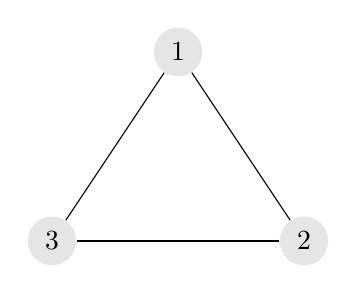
\begin{tikzpicture}
  [scale=.8,auto=left,every node/.style={circle,fill=gray!20}]
  \node (n1) at (5,5) {1};
  \node (n2) at (7,2)  {2};
  \node (n3) at (3,2)  {3};

  \foreach \from/\to in {n1/n2,n1/n3,n2/n3}
    \draw (\from) -- (\to);
\end{tikzpicture}
\caption{A network of three peers}
\label{fig:threepeers}
\end{figure}


\subparagraph{Firewall Problems}
In a test having one process running on a server in Internet and outside of the local network and having two
different processes running on one laptop but on different ports it is observed that the changes (sets) in the
Internet does not replicate to the local processes but the changes from local processes are being replicated to the other process.

\subparagraph{conclusion}
Having a network between local and Internet processes in the above mentioned method is not reliable. 
Repeating the tests with only local processes which are bootstrapping to one of them and running the setter/getter
methods showed that even in this scenario it is not reliable and one can not guarantee that the desired value will be returned.


\subsection{Concoord}
Describe why it is not suitable for us. It allows single object sharing.

\section{Distributed Workflows}
In this section we introduce a number of existing scientific workflow systems.
\subsection{COSMOS}\cite{Gafni30062014}
\subsection{Weaver}\cite{Bui_weaver:integrating} % making readers familiar with state of the art, where to asses?
\chapter{Problem Analysis}
\label{cha:analysis}

There are a number of possible use cases in our problem domain. To demonstrate these cases we assume
we have a number of nodes and datasets respectively, but they are not necessarily on the same nodes.
In the following paragraphs we explain possible combinations of operations, nodes and datasets.

\section{Operation}
In every scenario we want to run an operation which could be linear or non-linear.

\subsection{Linear Operation}
Being linear means that the operation
could be broken into its components and then run in parallel or series. Here is algebic notation
of a linear operation which acts on two datasets:

\[ Operation(A + B) = Operation(A) + Operation(B) \]

Being linear or non-linear only matters when we have to operate on more that one dataset.

\subsection{Non-linear Operation}
In contrast to linear there is non-linear operation. This means that this kind of operation has dependant parts and
those parts could not run in parallel:

\[ Operation(A + B) \neq Operation(A) + Operation(B) \]

\section{Datasets}
For each operation we need one or more datasets which my be available on the same node that wants to run the operation
initially or could reside on other nodes. 

\subsection{Input}
Input files are normally not mission critical and could be reproduced.

\subsection{Output}
Operations create output datasets which normally are small in size, threfore we ignore the transfer cost of operation
results in our work.

\subsection{Data Locating}
We consider three different approaches toward preparing required data for operations.
\subsubsection{Conventional Approach}
in this approach we put the required data on a network file system and all
application instances will access it there. We will utilize an NFS mounted file system.
\subsubsection{Centralized Approach}
in this approach we will have a central instance which will orchestrate operation
delegation and operation output forwarding to other nodes.
\subsubsection{Decentralized Approach}
in this approach we will eliminate the orchestrator node and the network of
application instances should collaborate in a decentralized fashion to keep track of data and control flow for each
task.

For every approach we will run performance tests and we will compare the results.

\subsubsection{Method}
We will discuss scenarios in chapter\ref{cha:scenarios}. For each scenario we will analyze the possible combinations 
of data and operations and we will discuss how to 
deliver the input data and where to store output data. We will discuss workflow management in chapter 
\ref{cha:workflow} and data transfer in chapter\ref{cha:data}.


% TODO: I might need to introduce "Decision Tree"
\section{Decision Making}
The main decision that we need to make at every scenario is whether we should transfer the required data or we
need to delegate the operation to an instance on a node which already has the data. To make a decision we need to
answer a number of questions. First we need to know the location of the data:

\begin{enumerate}
\item Is the data available locally?
\item If not, is the data available on another node? -- Here only the physical location of data matters not the instance
controlling it.
\end{enumerate}

% TODO: Introduce "Decision Metrics"

%In case the mentioned data is available on another nodes we have to answer these questions:
%\begin{enumerate}
%\item What is the cost of data transfer? -- We have to invent an algorithm for this calculation
%\item If data is available on more than one remote node, which one has the minimum transfer cost? -- We might
%introduce multiple strategies and use some heuristics for this selection, simplest form would be random selection,
%another could be asking for an availability metric from the instance and mix it with local calculated availability 
%metric to get a final cost value.
% TODO: We can use "Heartbeat" concept as one of availability metrics
%\item In case it is expensive to transfer the data, can we delegate the operation to an instance on the other node?
%\end{enumerate}



\section{Concrete Scenarios}
We begin with a simple scenario and we gradually add details to it and build new scenarios.

\subsection{Scenario 1}
In this scenario we have a linear operation, e.g. \(Op^A\) on \(Node^A\) which
requires one single dataset such as \( Dataset^1 \) which is available on one of the other peers.

\subsubsection{Conditions} \( Dataset^1 \) is not available on \( Node^A \) and the operation is linear.
\subsubsection{Consequences} With these conditions we either should transfer \( Dataset^1 \)
to local node or in case of availability delegate \(Op^A\) to the node which already has \( Dataset^1 \).

\subsection{Scenario 1 (UC1)}
We have a distributed network of collaborating servers, where in this case, we consider two computers. 
Each server has its own storage and maintains a number of datasets on it. These servers collaborate 
together to accomplish issued commands. User in this case wants to perform one operation on a dataset
that resides only on one of the servers. There are two main assumptions here:
\begin{enumerate}
\item \textbf{The user has neither a prior knowledge where the data is stored}
\item \textbf{Nor of how many servers are present on the network}
\end{enumerate}

The user connects to one of the servers, which we call a client. This server is assumed to be part 
of the network, though it may not have any local data stores on it. The user issues, interactively
(or non-interactively) a command on a set of data providing some kind of identification. This command
is broadcast by the client to all servers in the network. All servers receive this command and check
whether they have the data locally. The server which has the data performs the operation and the others
ignore it. The result of the operation in this case, remains on the same server which the original 
dataset was on. 

\begin{itemize}
\item Note: it is assumed that at any instance of time, only one server acts as a client.
\end{itemize}

Moreover we assume the user has already queried the available data in the entire network by 
issuing something like “list datasets” which outputs dataset names and ids.

The following table shows two servers, each has one dataset. The user is connected to S2.\\

\begin{tabular}{ l c r }
\em{Server ID} & \em{ Dataset ID} & \em{ Client} \\
S1 & DS1 & No \\
S2 & DS2 & Yes \\
\end{tabular}\\

Let us assume the data sets are \(10^6\) random numbers.
Let us assume the operation is to transform the real random numbers to a set of [0 or 1 ] depending on whether the number is even or odd. 
This operation is assumed here to be a user defined method that operates on the data set.

\begin{itemize}
\item Note: A dataset can be for example defined as an object that has an id, and a one dimensional array (python list).
\end{itemize}

The user issues the command like this from a python shell: 

\begin{itemize}
\item real2bin(DS1) will result in -> Broadcast(real2bin(DS1))
\item Note: it is assumed that all functions are already defined on all servers, since they execute the same environment.
\end{itemize}

The client broadcasts this function to all servers. Each server will check if the data set with this id exists, if so will run the command. 

This means that each server, especially the client, has to “know about all data sets existing in all servers.
It does not need to have the actual data, but needs to know about it. So that when the user issues the command
above, he/she does not get a “data structure not existent” error from the client, just because the data is not
there. Hence we need some interface, or some wrapper function that checks the argument for the data type, or to 
create some proxy interface from all data to all nodes. 

\section{Assessing Suggested Approaches}
To be able to assess the performance of each given solution to the mentioned scenarios we made a demo application
called \textbf{Konsensus}. The code is available on Github. %TODO add ref here

\subsection{Testing Problems}
Writing tests for a distributed application is not as easy as writing unit-tests for a normal application. 
Our demo application acts as a server and client at the same time. Moreover we want to launch multiple 
network peers running on one or more machines. Testing scenarios on this network is not possible with
normal mocking approaches, because we need to test the behavior of our solution in a network of collaborating
peers which are not external, rather the core services of the application.

To overcome testing issues we have to launch the desired number of peers separately and then run our tests 
over them. To make this operation faster we changed the application to make it possible to launch any number
of instances on one machine and we automated this process using a number of scripts. %TODO more details

\subsubsection{Mixing Signals in Greenlets}
We use python Greenlets instead of threads. This means that our demo application runs on only one thread. 
This causes a problem when launching multiple apps all together with one script and inside one thread, that
causes the signals for events spread among all greenlets and make trouble. To avoid this we have to run
each server in a separate processes. Running them inside threads won't help as well because the blinker python
library is thread-safe so it moves signals between threads as well as Greenlets.

\subsection{Scenario 2 (UC2)}
This is similar to scenario one, except that the operation requires two datasets to be done. We have a network of peers collaborating
to finish some linear and non-linear tasks. In this scenario we need at least three peers involved. We assume the first peer has no
data of our interest therefore it should cooperate with others to accomplish the request. Our operation in this case requires two 
different datasets which are not available on the first peer and we should access them on other peers. The main points the same:

\begin{enumerate}
\item \textbf{The user has neither a prior knowledge where the datasets are stored}
\item \textbf{Nor of how many servers are present on the network}
\item \textbf{The operation is linear}
\end{enumerate}

We assume the data distribution is like the following table:

\begin{tabular}{ l c r }
\em{Server ID} & \em{ Dataset ID} & \em{ Client} \\
S0 & --- & Yes \\
S1 & DS1 & No \\
S2 & DS2 & No \\
\end{tabular}\\

\subsubsection{Possible Approach}
In order to calculate the result we might take a number of approachers, we start with a combination of \textbf{divide and conquer} and
\textbf{produce-consume-collect} methods.

The S0, in this case, is the peer who receives the command and initiates the request. The two other peers, S1 and S2 respectively, have the required
datasets. The initiator will find the corresponding datasets and will dispatch commands to run each part on each peer and then will collect
the resulting datasets. This will be a blocking operation, we will wait until the other peers finish their parts and return the result
to us. If the output is a number it will be returned to the user, if it is a dataset it will be stored based on defined storage mechanism, 
currently we use random storage. The peer will break the operation into smaller operations each one calculating result for one of datasets, 
this \textbf{sub-operations} will be executed like \textbf{scenario 1} and the result will be collected by initiator peer.

We assume that in this case we have two arrays, each consisting of \(10^6\) random numbers. We have to first transform these datasets into
a set of [0 or 1] based on the number being even or odd (use case 1) and then we make a third dataset which contains the sum of every two
corresponding numbers in range of [0 to 2].


\begin{itemize}
\item Note: in this case each pear should be able to run the requested linear operation on one or more datasets.
\end{itemize}

The notation of above mentioned approach will be like this:

\[ Operation(A + B) = Operation(A) + Operation(B) \]

In order to run this operation in a collective way, we need to think of the type of service calls in our system, whether they are blocking or
non-blocking. Since often the operations in HPC environments are time consuming and long-running, we consider the non-blocking approach. In
this way the user will provide a dataset name for storing the result. The operation will be \textbf{submitted} to the collaborative network.
Later on user is able to query for the result using the key that she had provided at the time of submission. This allows us to design our system
in a more decentralized way, where each peer can inform others (neighbors) about a request in a \textbf{publish-subscribe} manner, where the peer
will publish a request and finish the operation. Later on the peer who has the dataset will \textbf{react} to the published request and will take
further actions, all the other peers who do not have the requirements (the dataset for now) will ignore it, however they can store the details of 
running operations for next steps, when we will come to more complex workflow.

To show more detailed version of this operation we demonstrate the steps for it:

\begin{enumerate}
\item User issues the command to S0, providing DS1, DS2 \st{and a unique name for the result}
\item System will check whether the operation is linear
\item Then it will break the command into sub-commands, each for one of datasets
\item System will generate unique ids for each sub-command
\item System will then submit the sub-commands along with dataset name and the unique id for the result dataset
to \textbf{itself}, which will cause a situation like scenario 1
\item System will next have to collect the results in a non-blocking manner which we will discuss shortly.
\end{enumerate}

\begin{itemize}
\item With the use of operation ids we eliminate the need to get a result dataset name from user but we still can accpte \textbf{tags} from users.
\end{itemize}

\begin{itemize}
\item We assume every operation involving more than one dataset is made of other operations which are already defined in the system.
\end{itemize}

There is an important issue here, we create sub-operations for each operation and we run them in a non-blocking manner, this will
cause it almost impossible to return the result of operation to the user in one run. One might think that we can block and query
until the result of sub-operations are ready, but this is something that we want to avoid. Therefore to solve this issue in a 
distributed manner, we introduce an operation id for each user request. We inform all the peers via sending messages (signals) about
the new operation and it's id and sub-commands. Each peer will update this operation internally based on further received messages.
We also return the operation id to the user instead of any results. Then user will query for the result of operation, providing the 
operation id. We change the above steps like this:

\begin{enumerate}
\item User issues the command to S0, providing DS1, DS2 and a unique name for the result
\item \textbf{System will generate a unique id for the operation and will store it along with the parameters}
\item System will check whether the operation is linear
\item Then it will break the command into sub-commands, each for one of datasets
\item System will generate unique ids for each sub-command
\item \textbf{System will notify other peers about the incoming operation with related parameters}
\item System will then submit the sub-commands along with dataset name and the unique id for the result dataset
to \textbf{itself}, which will cause a situation like scenario 1
\item System will next have to collect the results in a non-blocking manner which we will discuss shortly.
\item System will return the operation id to the user
\end{enumerate}

In the other hand the other peers which are the same basically, will react to the new operation signal:

\begin{enumerate}
\item Receive operation update message
\item Make a local lookup if the operation should be added or updated
\item Add or update the operation in the local storage
\end{enumerate}

Having the operation id and local updating storage for operations we now need to find a way to collect the results.
First of all we need to decide which peer will collect the results. We take the most straigh forward for now, the 
initiator peer, which has the knowledge of existing datasets in the network along with their sizes, will pick the 
peer which contains the largest dataset as the collector peer. We explicitly decide about the collector node in the
beginning either by size or randomly amount the data container peers.

It is worthy to mention that the collector peer will then store the result based on the configured storage mechanism 
which is random storage for now, not necessarily storing on the same node.

Now we have enough information in each peer to collect, process and store the results. The peers (including the collector)
 will react to operation methods like this:

\begin{enumerate}
\item Receive operation update message
\item Make a local lookup if the operation should be added or updated
\item Add or update the operation in the local storage
\item Am I the collector? If yes do the followings:
\begin{itemize}
\item check if the sub-operations are done
\item If the sub-operations are done, collect their results
\item Process the results
\item Based on the storage mechanism store the result
\item Update the operation with the result dataset id
\item Change status of operation to "done" (we need a proper state-machine here)
\item Inform other peers about the update
\end{itemize}
\end{enumerate}

Now if user makes a query giving the operation id this would be the result:

\begin{enumerate}
\item Check operation storage
\item If the operation is marked done, return the dataset id
\item If it is not done, return the status.
\end{enumerate}

\section{Operation Implementation}
About implementation of operation decorator (aspect?)

\section{Observed Errors}
While testing scenario 2 we observed a common error. We this scenario with three different peers as the following table:

\begin{tabular}{ l c r }
\em{Server ID} & \em{ Dataset ID} & \em{ Client} \\
S0 & --- & Yes \\
S1 & DS1 & No \\
S2 & DS2 & No \\
\end{tabular}\\

We also used \textbf{Random Dataset Storage} mechanism, simply to store resulting dataset of one operation on one of the network
peers. The problem is when two peers decide to store the result of one operation on each other a blocking condition happens. Our
approach was opening a temporary port and inform the other peer to fetch the data. Meanwhile this is exactly happening on the other
peer, therefore both block.

\subsection{Solution}
To solve the blocking peers problem we used the already running main application API instead of opening temporary PULL/PUSH zeromq 
sockets. This change is working fine and the peers exchanging datasets with no problem.

\section{Show Cases}

In this chapter we will go through a set of experiments to showcase the result of taking different approaches toward file transfer techniques. Meanwhile we will try a number of data distribution methods to see how they fit into our scenarios.

\section{Distributed Hash Tables}
Distributed Hash Tables (DHT) known best for their application to build torrent tracking software, let us to have a key/value store and distributed it in a decentralized way amount a network of peers.

MORE INFO HERE ON DHT, KAMEDLIA PAPER and IMPLEMENTATIONS

In our case to keep track of the available data on the network of collaborating peers, we can use a DHT table. Every time an instance wants to find a dataset it should query the network of peers using one of the existing wrappers and implementations.

\section{Test Results}
Our tests show that even though DHT is fault-tolerant and reliable for file distribution, it is not adequate for our realtime requirement to find our required data. In one test we ran two peers, one on an Internet host and another one on local host. Here are the client and server codes:

\begin{python}
from twisted.application import service, internet
from twisted.python.log import ILogObserver

import sys, os
sys.path.append(os.path.dirname(__file__))
from kademlia.network import Server
from kademlia import log

application = service.Application("kademlia")
application.setComponent(ILogObserver, 
	log.FileLogObserver(sys.stdout, log.INFO).emit)

if os.path.isfile('cache.pickle'):
    kserver = Server.loadState('cache.pickle')
else:
    kserver = Server()
    kserver.bootstrap([("178.62.215.131", 8468)])
kserver.saveStateRegularly('cache.pickle', 10)

server = internet.UDPServer(8468, kserver.protocol)
server.setServiceParent(application)


# Exposing Kademlia get/set API
from txzmq import ZmqEndpoint, ZmqFactory, ZmqREPConnection,
 ZmqREQConnection

zf = ZmqFactory()
e = ZmqEndpoint("bind", "tcp://127.0.0.1:40001")

s = ZmqREPConnection(zf, e)

def getDone(result, msgId, s):
    print "Key result:", result
    s.reply(msgId, str(result))

def doGetSet(msgId, *args):
    print("Inside doPrint")
    print msgId, args

    if args[0] == "set:":
        kserver.set(args[1], args[2])
        s.reply(msgId, 'OK')
    elif args[0] == "get:":
        print args[1]
        kserver.get(args[1]).addCallback(getDone, msgId, s)
    else:
        s.reply(msgId, "Err")

s.gotMessage = doGetSet
\end{python}

In the above example we have used \textit{twisted} networking library\cite{TwistedMatrix} and one python implementation\cite{KademliaImpl} of \textit{Kademlia} DHT algorithm\cite{KademliaPaper}. This will start a p2p network and will try to bootstrap it with another peer on the give IP address. Thereafter it will open another endpoint to expose a simple \textit{get/set} method for the rest of application for communicating with the network.

HERE DESCRIBE ABOUT DHT IMPLEMENTATION AND TWISTED NETWORKING LIBRARY. ***MOST IMPORTANT*** ABOUT REPLICATION OF DATA, IS THERE ANY REPLICATION? WHAT IF A NETWORK NODE FAILS? ***RCP OVER UDP AND WORK THROUGH FIREWALLS***

The next part is a few lines of code to communicate with this network:

\begin{python}
#
# Request-reply client in Python
# Connects REQ socket to tcp://localhost:5559
# Sends "Hello" to server, expects "World" back
#
import zmq

# Prepare our context and sockets
context = zmq.Context()
socket = context.socket(zmq.REQ)
socket.connect("tcp://localhost:40001")

# Set request
socket.send(b"set:", zmq.SNDMORE)
socket.send(b"the key", zmq.SNDMORE)
socket.send(b"the value")
print socket.recv()

# Get request
socket.send(b"get:", zmq.SNDMORE)
socket.send(b"the key")
print socket.recv()

# Invalid get
socket.send(b"get:", zmq.SNDMORE)
socket.send(b"not existing")
print socket.recv()
\end{python}

This simple client will try to connect to the previously opened port and send get/set messages.

\subsection{The Problem}
Configuring this p2p network is a little tricky. The network should work correctly even if nodes enter and leave the network. During our tests in development environment we observed some problems with initializing the network, but while the network was initialized leaving and entering the network had no effect on the results.

\subsubsection{Reliability}
Having the number of nodes increased up to 3 the reliability shows up again. When we set a value for a key in one node we can not guarantee that getting the value for that key on other nodes will return the updated one. With a number of tests I can confirm that two nodes which are bootstrapped with the same third node does not provide the accurate result every time and it is not clear for me why this happens. See figure~\ref{fig:threepeers} on page ~\pageref{fig:threepeers}.

After running more tests, we figured out that the possible source of the above mentioned problems was the confusion in using \textit{binary} and \textit{string} in python, so it was an error in our side.

\begin{figure}
\centering
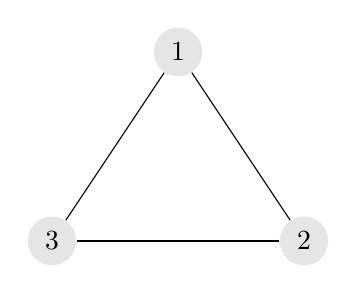
\begin{tikzpicture}
  [scale=.8,auto=left,every node/.style={circle,fill=gray!20}]
  \node (n1) at (5,5) {1};
  \node (n2) at (7,2)  {2};
  \node (n3) at (3,2)  {3};

  \foreach \from/\to in {n1/n2,n1/n3,n2/n3}
    \draw (\from) -- (\to);
\end{tikzpicture}
\caption{A network of three peers}
\label{fig:threepeers}
\end{figure}


\subsubsection{Firewall Problems}
In a test having one process running on a server in Internet and outside of the local network and having two different processes running on one laptop but on different ports it is observed that the changes (sets) in the Internet does not replicate to the local processes but the changes from local processes are being replicated to the other process.

\subsection{conclusion}
Having a network between local and Internet processes in the above mentioned method is not reliable. Repeating the tests with only local processes which are bootstrapping to one of them and running the setter/getter methods showed that even in this scenario it is not reliable and one can not guarantee that the desired value will be returned.


\section{Network Programming}
To showcase our desired approach and trying different ones we have used a number of network programming frameworks for python programming language. The main library that we use is called ØMQ or ZeroMQ~\cite{ZeroMQ}. ZeroMQ is an asynchronous messaging library written in C with bindings for many languages including python. This library helps us to easily scale and use different programming paradigms such as publish-subscribe, request-replay and push-pull.

\section{Publish-Subsribe Method}
Because of reliability issues we fall back to use a simpler approach using ZeroMQ. In this stage our aim is to distribute the information about available datasets at each node. To achieve this we let our demo application launch a number of communicators and publish information about it's data. Other nodes in our network have to subscribes on other nodes, hopefully ZeroMQ allows us to subscribe to multiple publishers, therefore each node can subscribe to other nodes. Nodes frequently get \textbf{news} from other nodes, for example availability of certain datasets on a node, then it can use publish-subscribe to get extra information on that particular subject.

\subsection{Architecture}
For demonstration purposes we create a python console application using Gevent\footnote{\url{http://www.gevent.org/}}, zeromq\footnote{\url{http://zeromq.org/}} and zerorpc\footnote{\url{http://zerorpc.dotcloud.com/}} to be able to service multiple requests in a non-blocking fashion.

\subsubsection{Application Initialization}
First of all each application instance establish its own zeromq publisher socket. Then it subscribes itself to all other nodes which are listed in config file. At this stage it should be configured manually.

\subsubsection{Gevent and non-blocking}
HERE WRITE ABOUT GEVENT.

\subsection{Exposing API}
Since this is going to be a network program we need to use a form of Remote Procedure Call (RPC) to communicate between nodes. Rather than implementing ourselves we used a library based on zeromq called \textit{zerorpc}. Using this library we now expose a set of APIs and let the nodes talk to each other based on this API. There are multiple solutions for exposing services which we do not discuss here.

\subsubsection{Data transfer using zerorpc}
WHICH DATA TYPES ARE WE ALLOWED TO TRANSFER USING ZERORPCS? IS IT ENOUGH FOR US?

\subsection{Application's State}
WE HAVE TO DECIDE ON A STATE MANAGER TO MAKE APPLICATION'S BEHAVIOR RELIABLE.

\subsection{Network Discovery}
At this stage there is no network discovery, because it is not our main problem. It can be done later as an improvement.

\subsection{Failure Recovery}
Again this is not of our interest. The point is there are existing solutions for these problems and we want to let our application to be able to demonstrate the main problem which would be deciding about data transfer routes and distributing the information about currently running operations.

\section{Use Case One Problems}
When we ask for an operation and we want to store the result somewhere on the network we have to think about the result name. 
We need a consistent way of naming datasets. If we ask users to provide resulting dataset names it will break soon, we need to 
let user to somehow give some \textbf{tags} but not the real names. We have to let the user know about the result name but also
let her to look for datasets by providing some tags.

The simplest problems that will happen if we store datasets with similar names is redundant work in the network. Peers will start 
to process and override the same dataset.

\subsection{Data Manipulation}
We will neet to let users to manipulate currently existing datasets, but very fast it comes to mind that not every dataset should be
writable, we will need to categorize and identify our datasets based on some criteria. These problems are not part of my thesis but
We mention it as part of problem analysis.



\section{Rough Ideas}

This chapter contains very raw ideas to address main requirements i.e.
distributed workflow management and intelligent data transfer.

\section{Intelligent Data Transfer: Use Case One}
By \textit{Intelligent Data Transfer} we mean an approach that
minimizes required data transfers between application\footnote{To be defined}
instances.

In the most basic use case\footnote{To be added later and 
referenced here} we run a script
\footnote{To be defined and added to
the terminology, terminology itself has to be defined}
which consists of two linear operations. Each operation consumes data
and generates data. A third operation needs both generated data two 
operate on and generate the third and final data.

The script is data driven. It means that it contains a number
of steps and for every step it needs appropriate data to run the
desired operations\footnote{To be defined}. We assume that
the script will run on \textit{Node 1} and required data 
\textit{DataSet1} and \textit{DataSet2} are 
located on \textit{Node 2}
and \textit{Node 3} respectively. Therefor \textit{Node 1} have
to initiate operations on the other machines.

\subsection{Identical Instances}
We assume that on each machine of the network the same instance of our program is running which 
is capable of all of our operations
including A, B and C. The only consideration is the availability of 
Datasets, they are not available on all machines.

A linear operation (not clear to my self how to write it):

\[ Operation(A, B) = Operation(A) + Operation(B) \]

\[ DataSet^A = Operation^A(DataSet^1) \]

\[ DataSet^B = Operation^B(DataSet^2) \]

\[ DataSet^C = Operation^C(DataSet^A, DataSet^B) \]

Assuming that operations A and B will run on the machines which
contain the required data, a number of questions arise here:
\begin{enumerate}
\item On which machine operations C should run? A, B or C?
\item On How to transfer the required data to that machine in an 
optimized way?
\end{enumerate}

\subsection{The Idea}
First of all we assume that we have the information about the Datasets
available on all of the machines i.e. in form of a distributed table
with entries containing the node address and Dataset id. Based on this
information the application can decide if it has the required data or
not. 

Based on this algorithm (to be defined) the initial application
delegates operations to the other nodes (instances of the same program),
where the data is available. Our distributed workflow manager (to be 
defined) will synchronize the information on these running operation and
will label the output data and will add it to the distributed data table.

After finishing operations A and B we will run operation C in either
of these nodes, because the required data is partially available on these
nodes. Then we have to transfer the rest of the data to one of these
nodes to run the operation C which needs both parts simultaneously.

\subparagraph{Using Prior Art}
At this point we can take advantage of existing Distributed File Systems
(DFS) to make the data available for operation C. We can then eliminate
the complexity of data transfer between these two nodes and delegate it
to existing distributed file systems. The main point is we don't rely on
DFS for all of our decision making part but we explicitly make the 
decision to run operation A and B on specific nodes and then for the 
last part we use a meta or universal disk concept to deliver the
remaining data for operation C.

\section{Sqmpy Integration}
We can use Sqmpy project as a monitoring tool for konsensus network.
 Providing one peer address it can query the rest of peers and connect or 
subscribe to their news channel. Having this we can always see which nodes are
offline and which ones are online. This also gives us a platform to extend
monitoring and control features to the web. Currently we have made all the 
required software platform to achieve this. On Sqmpy side using Flask microframework
and socket.io we can simply maintain realtime connections to the browsers and since
our web framework is written in python, with minimum cost we can integrate it
with konsensus.
 % problem analysis
\chapter{Proposed Solution}
\label{cha:proposal}
In this chapter we explain how we can solve the scenarios which we explained in previous chapter.
We introduced seven different scenarios, three of them for linear operations and three of them for non-linear
ones, and one mixed operation type. We begin with the most basic scenario, solving a data intensive operation
which requires one dataset. Then we will extend it to accept more datasets and we will sove them. We will
cover only solving linear operations and non-linear operations will be left for further work.

\section{Basic Idea}
The basic idea that we will follow in this chapter, relies on breaking the operations into smaller units which
we can solve them in one separate step, such as only one operatino call or service call. 
The building blocks for complex operations are the simple operations.
We build them on top of the atomic units, which we know how to solve them.

We assume that we have the information about the datasets
available on all machines i.e. in form of a distributed table
with entries containing the node address and dataset id. Based on this
information the application can decide if it has the required data or
not. We will explain this in detail later in this and next chapter.

Based on this algorithm the application implicitly delegates operations to the other 
nodes (instances of the same program), where the data is available. It would be a non-blocking service call, 
just like signaling others about an incoming request.
Along with any operation change, the distributed workflow manager will synchronize the information amoung the peers.
Any change in datasets in any collaborative node will also be synchronized with peers and will be added to 
a distributed list.

\subsection{Break and Conquer}
\subsection{Recursive Call}
\subsection{Collectors}
\subsection{Asynchronous Calls}
\subsection{Unique IDs}


\section{Operation Types}
\subsection{Simple Operation}
\subsection{Mixed Operation}

\section{Using Prior Art}
\subsection{Data Transfer}
We can take advantage of existing Distributed File Systems
(DFS) to make the data available for operations. We can then eliminate
the complexity of data transfer between these two nodes and delegate it
to existing distributed file systems. The main point is we don't rely on
DFS for all of our decision making part but we explicitly make the 
decision which operations to run on specific nodes and then for the 
data transfer part we can use a meta or universal disk concept to deliver the
remaining data.


% ==============================================
% ==============================================
\section{Proposed Approach}
In order to calculate the result we might take a number of approachers, we start with a combination of \textbf{divide and conquer} and
\textbf{produce-consume-collect} methods.

The S0, in this case, is the peer who receives the command and initiates the request. The two other peers, S1 and S2 respectively, have the required
datasets. The initiator will find the corresponding datasets and will dispatch commands to run each part on each peer and then will collect
the resulting datasets. This will be a blocking operation, we will wait until the other peers finish their parts and return the result
to us. If the output is a number it will be returned to the user, if it is a dataset it will be stored based on defined storage mechanism, 
currently we use random storage. The peer will break the operation into smaller operations each one calculating result for one of datasets, 
this \textbf{sub-operations} will be executed like \textbf{scenario 1} and the result will be collected by initiator peer.

We assume that in this case we have two arrays, each consisting of \(10^6\) random numbers. We have to first transform these datasets into
a set of [0 or 1] based on the number being even or odd (use case 1) and then we make a third dataset which contains the sum of every two
corresponding numbers in range of [0 to 2].


\begin{itemize}
\item Note: in this case each pear should be able to run the requested linear operation on one or more datasets.
\end{itemize}

The notation of above mentioned approach will be like this:

\[ Operation(A + B) = Operation(A) + Operation(B) \]

In order to run this operation in a collective way, we need to think of the type of service calls in our system, whether they are blocking or
non-blocking. Since often the operations in HPC environments are time consuming and long-running, we consider the non-blocking approach. In
this way the user will provide a dataset name for storing the result. The operation will be \textbf{submitted} to the collaborative network.
Later on user is able to query for the result using the key that she had provided at the time of submission. This allows us to design our system
in a more decentralized way, where each peer can inform others (neighbors) about a request in a \textbf{publish-subscribe} manner, where the peer
will publish a request and finish the operation. Later on the peer who has the dataset will \textbf{react} to the published request and will take
further actions, all the other peers who do not have the requirements (the dataset for now) will ignore it, however they can store the details of 
running operations for next steps, when we will come to more complex workflow.

To show more detailed version of this operation we demonstrate the steps for it:

\begin{enumerate}
\item User issues the command to S0, providing DS1, DS2 \st{and a unique name for the result}
\item System will check whether the operation is linear
\item Then it will break the command into sub-commands, each for one of datasets
\item System will generate unique ids for each sub-command
\item System will then submit the sub-commands along with dataset name and the unique id for the result dataset
to \textbf{itself}, which will cause a situation like scenario 1
\item System will next have to collect the results in a non-blocking manner which we will discuss shortly.
\end{enumerate}

\begin{itemize}
\item With the use of operation ids we eliminate the need to get a result dataset name from user but we still can accept \textbf{tags} from users.
\end{itemize}

\begin{itemize}
\item We assume every operation involving more than one dataset is made of other operations which are already defined in the system.
\end{itemize}

There is an important issue here, we create sub-operations for each operation and we run them in a non-blocking manner, this will
cause it almost impossible to return the result of operation to the user in one run. One might think that we can block and query
until the result of sub-operations are ready, but this is something that we want to avoid. Therefore to solve this issue in a 
distributed manner, we introduce an operation id for each user request. We inform all the peers via sending messages (signals) about
the new operation and it is id and sub-commands. Each peer will update this operation internally based on further received messages.
We also return the operation id to the user instead of any results. Then user will query for the result of operation, providing the 
operation id. We change the above steps like this:

\begin{enumerate}
\item User issues the command to S0, providing DS1, DS2 and a unique name for the result
\item \textbf{System will generate a unique id for the operation and will store it along with the parameters}
\item System will check whether the operation is linear
\item Then it will break the command into sub-commands, each for one of datasets
\item System will generate unique ids for each sub-command
\item \textbf{System will notify other peers about the incoming operation with related parameters}
\item System will then submit the sub-commands along with dataset name and the unique id for the result dataset
to \textbf{itself}, which will cause a situation like scenario 1
\item System will next have to collect the results in a non-blocking manner which we will discuss shortly.
\item System will return the operation id to the user
\end{enumerate}

In the other hand the other peers which are the same basically, will react to the new operation signal:

\begin{enumerate}
\item Receive operation update message
\item Make a local lookup if the operation should be added or updated
\item Add or update the operation in the local storage
\end{enumerate}

Having the operation id and local updating storage for operations we now need to find a way to collect the results.
First of all we need to decide which peer will collect the results. We take the most straight forward for now, the 
initiator peer, which has the knowledge of existing datasets in the network along with their sizes, will pick the 
peer which contains the largest dataset as the collector peer. We explicitly decide about the collector node in the
beginning either by size or randomly amount the data container peers.

It is worthy to mention that the collector peer will then store the result based on the configured storage mechanism 
which is random storage for now, not necessarily storing on the same node.

Now we have enough information in each peer to collect, process and store the results. The peers (including the collector)
 will react to operation methods like this:

\begin{enumerate}
\item Receive operation update message
\item Make a local lookup if the operation should be added or updated
\item Add or update the operation in the local storage
\item Am I the collector? If yes do the followings:
\begin{itemize}
\item check if the sub-operations are done
\item If the sub-operations are done, collect their results
\item Process the results
\item Based on the storage mechanism store the result
\item Update the operation with the result dataset id
\item Change status of operation to "done" (we need a proper state-machine here)
\item Inform other peers about the update
\end{itemize}
\end{enumerate}

Now if user makes a query giving the operation id this would be the result:

\begin{enumerate}
\item Check operation storage
\item If the operation is marked done, return the dataset id
\item If it is not done, return the status.
\end{enumerate}
 % explaining the proposed design/algorithm
\chapter{Prototype}
\label{cha:prototype}

\section{Architecture}
In a traditional approach toward application layering we would have three tiers, i.e. client layer (GUI),
business layer (logic) and database layer. These tiers correspond to a one dimentional application architecture,
where there are only two \textit{sides} assumed to exist around application logic, client and database. However
this is not the case when we have a multi-dimentional architecture, where there are multiples input/output channels
around our business logic. In the latter case we have to use a so called hexagonal architecture. \cite{alistair}
In such an architecture applications receive signals from multiple communication means at the same time. This 
signals will trigger the appropriate internal business logic, therefore they can't be layered in one dimention.
\subsection{Overview}

\subsection{Actors}
There are two types of actors in our problem domain.
\subparagraph{User}
A user who launches, control and monitor an operation.
\subparagraph{Instance}
Every instance can launch and observe an operation on other instances on other nodes.
\subsection{Messaging}
\subsubsection{Publish/Subscribe}
\subsubsection{Filtering}
\subsection{Coupling}
\subsection{State}

\section{Technology}
We have created a python application using Gevent\footnote{\url{http://www.gevent.org/}},
zeromq\footnote{\url{http://zeromq.org/}} and zerorpc\footnote{\url{http://zerorpc.dotcloud.com/}} 
to be able to service multiple requests in a non-blocking way.

\subsection{Programming Language}
We select Python as the main programming language to implement this project. There are a number of 
justifications to do so. Here are the main ones:

\subparagraph{Multi-Platform} Python is a multi-platform language. It runs on different operating systems
seamlessly, hence easier deployment.
\subparagraph{High Availability} Python along with its rich standard library is available by default on almost all Linux machines. This
is a great advantage for use, because we do not need to take further steps to install a runtime in highly conservative institutes.
\subparagraph{Familiarity} Python is already being used as main scripting languages in many scientific environments. This would be an advantage
for us in further steps when users want to contribute to the project or maintain it.
\subparagraph{Based on C} Python is well known to be very close to C programming languages. Even though Python is slow in arithmatic operations
it is possible to write speed critical parts in C and execute it directly within Python code. However in our current solution we do not have
arithmatic operations.
\subparagraph{Faster Development} Since Python does not need special tools to build and deploy its scripts it is much cheaper and faster
to start, build and test programs.
\subparagraph{Aspect Oriented Support} With Python it is very easy to wrap methods and apply pre-process and post-process conditions to them. We have
used this aspect of the language to create operation ids, delegate service calls, distribute messages and etc before and after service calls.

\subsection{Dependency Management} Using \textit{pip}\footnote{\url{https://pypi.python.org/pypi/pip}}
it is very trivial to manage and install multiple
dependencies of a project. It is capable of installing dependencies from remote git repositories or from 
the Python Package Index (PyPI)\footnote{\url{https://pypi.python.org/pypi}}. Moreover \textit{pip} itself is
a Python package. It gives us huge benefits with abstracting away the complexity of dependency management. It can
bundle a package with compiled dependencies, install from Python wheel\footnote{A built-package format for Python}, uninstall,
upgrade and query available PyPI packages.\footnote{\url{https://pip.pypa.io/en/latest/user_guide.html\#create-an-installation-bundle-with-compiled-dependencies}}

\subsection{Virtual Environment}
As described in the previous section, Python is the chosen programming language for this project. Along with Python, 
comes \textit{virtualenv} package\footnote{virtualenv is a tool to create isolated Python environments}. This is a great way of installing
project dependencies into a single directory (which serves as the virtual root file system) and avoid touching operating system managed files and
directories which normal users do not have access to them. While working inside a \textit{virtaulenv}, all the changes is written to a single directory
and all binary files, downloaded Python packages goes into that directory. Therefore this is the best way to deploy a Python project in user space.

\subsection{ØMQ}
The main library that powers our prototype is called ØMQ or ZeroMQ~\cite{ZeroMQ}.
ZeroMQ is an asynchronous messaging library written in C with 
bindings for many languages including python. This library helps us to easily scale and use 
different programming paradigms such as publish-subscribe, request-replay and push-pull.

\section{Compoenents}
\subsection{Distributed Storages}
Our aim is to distribute the information about available datasets and operations at each node. To achieve this
we let our application to launch a number of communicators and publish information about it is data.
Other nodes in our network have to subscribes on other nodes, ZeroMQ allows us to subscribe
to multiple publishers, therefore each node can subscribe to other nodes. Nodes frequently get
\textbf{news} from other nodes, for example availability of certain datasets on a node, then it
can use publish-subscribe to get extra information on that particular subject.
\subsubsection{Operation Store}
\subsubsection{Dataset Store}
\subsection{Message Handlers}
\subsection{Decorators}
\subsection{Application}

\section{Layers}
\subsection{Network}
\subsubsection{API}
Since this is going to be a network program we need to use a form of Remote Procedure Call (RPC) 
to communicate between nodes. Rather than implementing ourselves we used a library based on zeromq 
called \textit{zerorpc}. Using this library we now expose a set of APIs and let the nodes talk to 
each other based on this API. There are multiple solutions for exposing services which we do not discuss here.
\subsubsection{Publisher}
\subsubsection{Listener}
\subsection{Pre-processing}
\subsubsection{Incoming Messages}
\subsubsection{API Calls}
\subsection{Backend}
\subsubsection{Logic}
\subsubsection{Stores}
\subsubsection{Database}

\section{Initialization}
First of all each application instance establish its own zeromq publisher socket. Then it subscribes
itself to all other nodes which are listed in config file.
\subsection{Local Database}
\subsection{Stores}
\subsection{Network}

\section{Control Flows}
\subsection{API Call Flow}
\subsubsection{Possible Reactions}
\subsection{Incoming Message Flow}
\subsubsection{Possible Reactions}

\section{Deployment}
The software is easily installable in a Python Virtual Environment.

\section{Test Results}
To be able to assess the performance of each given solution to the mentioned scenarios we made a demo application
called \textbf{Konsensus} which its code is available on Github. \cite{konsensus}

\subsection{Integration Tests}
Writing integration tests for a distributed application is not as straightforward as writing unit-tests for a normal application. 
Our demo application acts as a server and client at the same time. Moreover we want to launch multiple 
network peers running on one or more machines. Testing scenarios on this network is not possible with
normal mocking approaches, because we need to test the behavior of our solution in a network of collaborating
peers which are not external, rather the core services of the application.

To overcome testing issues we have to launch the desired number of peers separately and then run our tests 
over them. To make this operation faster we changed the application to make it possible to launch any number
of instances on one machine and we automated this process using a number of scripts. %TODO more details

\subsubsection{Mixing Signals in Greenlets}
We use python Greenlets instead of threads. This means that our demo application runs on only one thread. 
This causes a problem when launching multiple apps all together with one script and inside one thread, that
causes the signals for events spread among all greenlets and make trouble. To avoid this we have to run
each server in a separate processes. Running them inside threads won't help as well because the blinker python
library is thread-safe so it moves signals between threads as well as Greenlets.

\subsubsection{Scnenario 2 Errors}
While testing scenario 2 we observed a common error. We this scenario with three different peers as the following table:

\begin{tabular}{ l c r }
\em{Server ID} & \em{ Dataset ID} & \em{ Client} \\
S0 & --- & Yes \\
S1 & DS1 & No \\
S2 & DS2 & No \\
\end{tabular}\\

We also used \textbf{Random Dataset Storage} mechanism, simply to store resulting dataset of one operation on one of the network
peers. The problem is when two peers decide to store the result of one operation on each other a blocking condition happens. Our
approach was opening a temporary port and inform the other peer to fetch the data. Meanwhile this is exactly happening on the other
peer, therefore both block.

\subparagraph{Solution}
To solve the blocking peers problem we used the already running main application API instead of opening temporary PULL/PUSH zeromq 
sockets. This change is working fine and the peers exchanging datasets with no problem.
 % about the implementation details and techniques
\chapter{Discussions}
\label{cha:discussions}

\section{Possible Issues}
\subsection{High Load}
\subsection{Orphan Operations}
\subsection{Complexity Growth}

\subsection{Large Dataset Transfer}
To transfer large arrays over the network there are a number of considerations. Should the array be stored locally before transfer?
What if the array is so big that it does not fit into the machines memory? And how the array should be transferred?

Currently we assume the result datasets fit into memory, therefore there is only the question of how 
to transfer them over the network. To prevent unnecessary copies, we consider streams to send them to
other peers. In the demo application this is done with streaming sockets. The other peer will be notified and then it will fetch the desired dataset.

We need to develop a mechanism to consider dataset size for transfer. User defined files are normally small and we can safely transfer them but
system datasets are large and for any transfer some sort of control should happen. % discussing possible issues and future works
\chapter{Conclusion}
\label{cha:conclusion}

Even though there are many solutions designed for HPC problems, still there are requirements for smaller groups which are not satisfied, such as:
\begin{itemize}
\item Making scientific applications user friendly 
\item Providing \textit{smarter} solutions which get out of users way, i.e. hiding the systems complexity from ordinary users
\item The system manages data endpoints, not users
\item Less deployment and maintenance cost
\item More flexibility to control application at runtime
\end{itemize}
During this work we addressed some of these needs:
\begin{itemize}
\item The problem was defined and requirements where defined
\item We went through the state of the art
\item A solution approach was proposed
\item A prototype was developed
\begin{itemize}
\fontsize{30pt}{31}\selectfont
\item Based on open technologies
\item Runs in user space
\item Open source and freely available on Github
\end{itemize}
\end{itemize}
Our approach is very flexible to be extended and it is easy to build new services on top of the existing framework 
which provides the distributed operation and storage mechanisms to applications.

\section{Future Work}
During this work we have focused on the aspects of the problem which were important in the context 
domain and we left aside many other small and big problems without considering them during this project. The main
reason was that we wanted to work on problems which were new and genuine
because for other aspects there are already many well-defined solutions
available, so we did not spend our time for them. Moreover one should 
consider that this project is not solely an implementation but is a 
research on finding ways to embed distributed solutions into other projects.

In the following sections we talk shortly about the topics which we have
not covered but this work can be extended to include them as well.

\section{Non-linear Operations}
The main part which have not been covered yet is non-linear operations.


\section{Network Discovery}
Currently the peers are configured in the beginning and there is no dynamic peer recognition. This might be done in a number of ways
such as sending broadcasts or using third party projects such as Zyre \cite{Zyre}.

\section{Bootstrapping}
With having address of only one peer we would be able to configure and a new peer and join the network. There should be a mechanism among
peers to identify joining and leaving peers. But our context is different than a peer-to-peer applications which peers join and leave 
frequently. In our case most of peers run a long time and bootstrapping is more a way to get the state of currently running workflows and
let others know about the new peer.

\section{Data Popularity}
There are algorithms developed to calculate data popularity over time and then replicate them over peers for easier access. If we want to 
move toward any type of data replication we would need to use this algorithms.

\section{Security}
There is no user management and secure communication in our initial requirements however this would be required if we want to manage user
rights or introduce limitations or simply to keep a history of activities for each user. Moreover to secure inter-peer communications 
we might use X.509 certificates. Further more since we've used ZeroMQ\cite{ZeroMQ} as underlying transport channel we can use its more advanced
security features such as Elliptic curve cryptography\cite{Curve} based on Curve25519\cite{Curve25519} to add perfect forward secrecy, 
arbitrary authentication backends and so on.

\section{Fault Tolerance}
In current work there is no failure recovery mechanism, since it was not part of the requirements. In case of a failure or exception in any 
collaborating peer not only the failed instance should be able to recover itself into a correct state, moreover the other peers should maintain
a valid state for on-going distributed workflows and keep their internal state up-to-date. % thesis conclusion and future work


\printbibliography[heading=bibintoc, title={References}]

\end{document}